% Program : XeLaTeX
\documentclass[a4paper,11pt]{article}
    \usepackage[left=3cm,right=3cm,top=3cm,bottom=3cm]{geometry}
\usepackage{kotex}
\usepackage{indentfirst}
\usepackage[onehalfspacing]{setspace}
\usepackage{anyfontsize}
\usepackage{blindtext}
\usepackage{listings}
\usepackage[shortlabels]{enumitem}
\usepackage[bookmarks=true,pdfborder={0 0 0}]{hyperref}
\usepackage{graphicx}
\setmainhangulfont{UnBatang}

\renewcommand{\contentsname}{\center목 차}
\renewcommand{\listfigurename}{\center그림 목차}
\renewcommand{\listtablename}{\center표 목차}
\renewcommand{\abstractname}{\centering\noindent\fontsize{12}{\baselineskip} \selectfont{\textbf{개 요}} \vspace*{1cm}}
\renewcommand{\figurename}{그림}
\renewcommand{\tablename}{표}

\makeatletter
\renewcommand\maketitle{
{\raggedright % Note the extra {
\begin{center}
{\fontsize{14}{\baselineskip} \selectfont \@title }\\[1.5cm]
{\fontsize{12}{\baselineskip} \selectfont \@author}\\[1cm]
{부산대학교 공과대학}\\[1.5cm]
\end{center}}} % Note the extra }
\makeatother

\lstset{frame=tb,
  language=C,
  aboveskip=3mm,
  belowskip=3mm,
  showstringspaces=false,
    basicstyle=\normalsize,  % 2019 소스 글자크기 조정 함
    numbers=left,
    stepnumber=5,  % 점프 사이즈
    showstringspaces=false,
    tabsize=1,
    breaklines=true,
    breakatwhitespace=false,
  columns=flexible,
  basicstyle={\normalsize\ttfamily},
  numberstyle=\small\color{blue},
  keywordstyle=\color{blue},
  commentstyle=\color{teal},
  stringstyle=\color{magenta},
  breaklines=true,
  breakatwhitespace=true,
  tabsize=3
}

\title{\textbf{3조 텀프로젝트 최종 보고서 : 전자 피아노}}
\author{김동규, 김현수, 배준혁, Damir Assanov}
\date{\today}

\begin{document}

\begin{titlepage}
\vspace{4.5cm}
\makeatletter
\begin{center}
\noindent{\fontsize{16}{\baselineskip} \selectfont \textbf{임베디드 시스템 설계 및 실험}}\\[2cm]
{\fontsize{22}{\baselineskip} \selectfont \textbf{\@title}}

\vspace{7cm}

{\fontsize{12}{\baselineskip} \selectfont 2019년 12월 24일}

\vspace{1cm}
\begin{spacing}{1.6}
{\fontsize{16}{\baselineskip} \selectfont 김동규(201527506)}\\
{\fontsize{16}{\baselineskip} \selectfont 김현수(201424442)}\\
{\fontsize{16}{\baselineskip} \selectfont 배준혁(201424465)}\\
{\fontsize{16}{\baselineskip} \selectfont Damir Assanov(201624630)}
\end{spacing}

\vspace*{2cm}

{\fontsize{16}{\baselineskip} \selectfont 2019 임베디드시스템설계 및 실험\\목요일(004)분반 제3조}\\[2cm]
{\fontsize{16}{\baselineskip} \selectfont 2019년 12월 24일}

\vspace{4cm}

\end{center}
\makeatother
\end{titlepage}
%=================================================================
\vspace{3.5cm}
\pagenumbering{roman}
\maketitle
\addcontentsline{toc}{section}{개요}
\begin{abstract}
\begin{spacing}{1.6}
  이 프로젝트는 임베디드 시스템을 이용하여 전자 피아노를 구현한다. STM32F107VCT6보드와 압력센서, 디지털 앰프 모듈, 스피커를 이용하여 시스템을 구성하고 모든 구성품을 피아노 박스를 이용하여 정리, 건반을 입력 할 수 있는 피아노를 구현하였다. 건반 입력의 조합으로 function key를 사용, 피아노의 모드를 변경할 수 있고 녹음, 재생 기능을 지원한다.

\end{spacing}
\end{abstract}
\textbf{Keyword} \textit{PWM, DMA, ADC, LCD, Interrupt}
\newpage
\tableofcontents
\addcontentsline{toc}{section}{목차}
\listoffigures
\addcontentsline{toc}{section}{그림 목차}
\newpage
\pagenumbering{arabic}
\setcounter{page}{1}
%------------------------------------------------------
\begin{spacing}{1.6}
\section{목적과 배경지식}
\subsection{목적}
본 프로젝트는 임베디드시스템 설계 및 실험 수업을 통해 배운 지식을 활용하여 직접 프로젝트를 구현하며 학습내용을 복습하고 실제 임베디드 시스템 설계능력의 향상을 목표로 한다.
\subsection{배경지식}
\subsubsection{PWM}
Pulse-Width Modulation, PWM은 Duty의 비율을 제어하여 평균 전압을 조절하는 방법이다. 주로 LED와 같은 조명제품이나 DC모터의 제어에 사용되며 이번 프로젝트에 사용되는 스피커 역시 타이머를 통해 얻은 PWM값을 통해 소리를 출력한다.

\subsubsection{디지털 앰프}
디지털 앰프란 신호를 디지털 상태에서 증폭하는 앰프를 의미한다. 디지털 앰프는 음향 신호를 PWM신호로 변경, 이를 증폭하고 이후 PWM 신호를 Low Pass Filter 를 이용하여 원래의 아날로그 신호로 만들어낸다. 디지털 앰프는 아날로그 증폭회로에 비하여 신호 왜곡에 강하고 효율적이다.

\section{프로젝트 시나리오와 변경사항}
 \subsection{프로젝트 시나리오}
 피아노 프로젝트의 동작 시나리오와 프로젝트 구상시와 비교해 달라진 점을 설명한다.
 \begin{itemize}
   \item  첫 실행시 idle 모드로 시작한다.
   \item  피아노의 건반을 누르면 연결된 압력센서를 통해 ADC값을 얻고 해당 값이 경계값보다 클 경우 소리를 출력한다.
   \item  건반 입력의 조합을 통해 function key를 구현하였다. 이를 통해   Record 모드와 Play모드를 선택할 수 있으며 옥타브 변경이 가능.
   \item  Record 모드에서는 입력받은 건반을 기억하여 사용자 정의 배열에 저장한다.
   \item  Play 모드에서는 배열을 통해 사용자가 연주한 음악을 재생한다.
 \end{itemize}

 \subsection{변경사항}
 \begin{itemize}
   \item 옥타브 변경 기능은 조이스틱이 아닌 건반 입력의 조합, 즉 function key를 통해 구현함.
   \item 파일 시스템을 이용하는 외부 저장장치 대신 메모리에 구조체 배열을 통해 입력을 저장하도록 변경하였다.
   \item 하드웨어 코덱 대신 디지털 앰프 모듈을 이용하여 스피커와 시스템을 연결하였다.
   \item 저장소의 파일을 읽어 미리 저장된 음을 출력하는 대신 PWM신호를 통해 음계를 출력.
   \item LCD는 출력용으로만 사용.
 \end{itemize}

\section{텀프로젝트 설계}
\subsection{필요 장비와 준비물}
  이 실험을 위해서는 다음의 준비물이 필요하다.
 \begin{itemize}
   \item STM32F107VCT6 칩셋
   \item STM32F107VCT6 데이터시트 1부
   \item STM32F107VCT6 참조 매뉴얼 1부
  \item PC, 모니터 각 1대(Windows 10, amd64)ㅈ
  \item DSTREAM 1대
  \item 점프케이블
  \item DS-5 Compiler / Debugger
  \item STM32F107VCT6 Library
  \item Flashclear Firmware : Flash 영역에 빈 코드를 Load하여 갱신 전에 펌웨어 삭제.
  \item Scatter File
  \item Configure Database
  \item 오실로스코프
  \item 만능기판
  \item 압력센서 12개
\begin{figure}[hbt!]
\centering
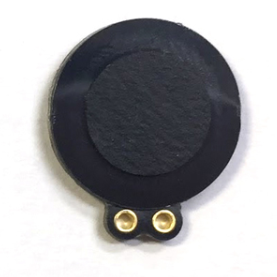
\includegraphics[scale=0.5]{m1.png}
\caption{압력 센서}
\label{Fig:Fig01}
\end{figure}

  \item 디지털 앰프 모듈
\begin{figure}[hbt!]
\centering
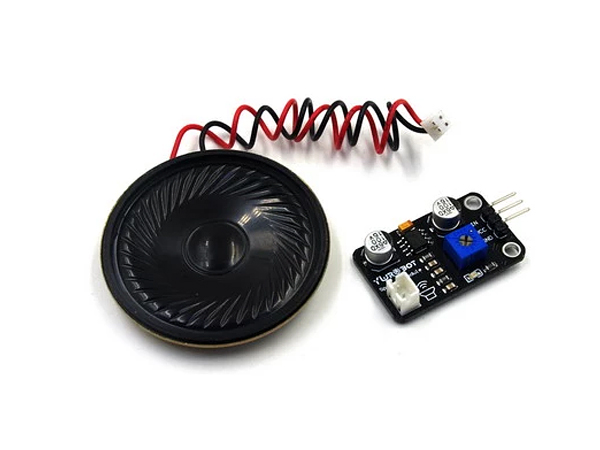
\includegraphics[scale=0.45]{m2.jpg}
\caption{디지털 앰프 모듈}
\label{Fig:Fig02}
\end{figure}

  \item 스피커
\begin{figure}[hbt!]
\centering
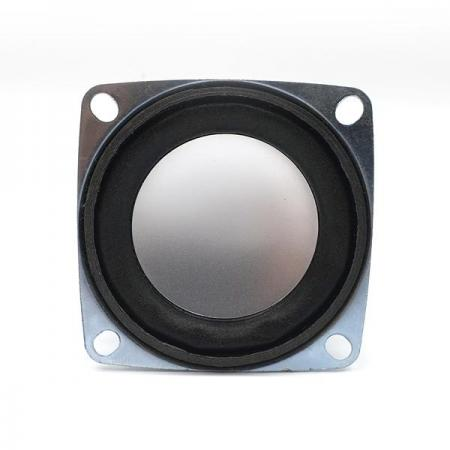
\includegraphics[scale=0.5]{m3.jpg}
\caption{4옴 임피던스 스피커}
\label{Fig:Fig03}
\end{figure}

 \end{itemize}
 \paragraph{일러두기} 이 절 이하에서 ``STM32F107VCT6 칩셋"은 ``임베디드 시스템"으로 칭한다.
\subsection{프로젝트환경 구성}
\begin{enumerate}
\item 만능기판에 압력센서 브릿지를 이용하는 회로를 구성하여 납땜한다. 납땜을 할 때는 중금속과 열을 이용하므로, 안전에 신경을 쓰도록 한다.

\begin{figure}[hbt!]
\centering
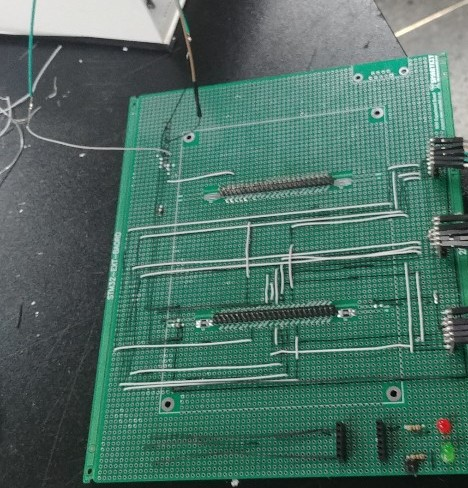
\includegraphics[scale=0.5]{1.jpg}
\caption{만능 기판 납땜}
\label{Fig:Fig04}
\end{figure}

\item 이후 만능기판을 보드에 연결한다. 만능기판의 압력센서 브릿지는 피아노 박스의 압력센서와 연결되도록 회로를 구성한다.
\begin{figure}[hbt!]
\centering
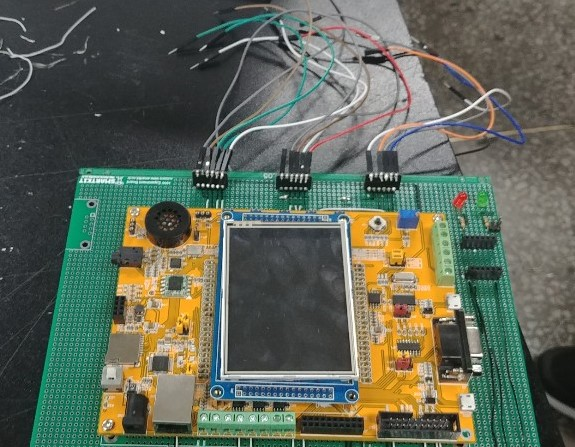
\includegraphics[scale=0.5]{2.jpg}
\caption{만능기판과 보드 연결}
\label{Fig:Fig05}
\end{figure}

\item 마지막으로  모든 구성품을 그림\ref{Fig:Fig03}과 같이 피아노 박스에 조립한다. 또한 보드의 위치를 조정하기위해 받침대를 추가하였다.
\begin{figure}[hbt!]
\centering
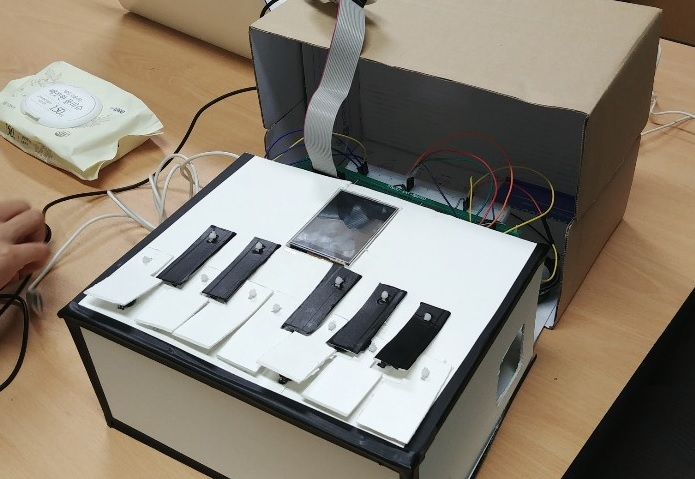
\includegraphics[scale=0.5]{3.jpg}
\caption{피아노 박스 조립}
\label{Fig:Fig06}
\end{figure}
\end{enumerate}

\section{소프트웨어 구현}
 \subsection{main}

 \subsection{건반 입력 구현}
 \subsection{녹음, 재생 기능}
 
\subsection{라이브러리 작성과 활용}
 효율적이고 확장 가능한 프로그래밍을 위하여 라이브러리 파일을 생성하였다.
 

\section{결론}
   이 실험으로 임베디드 시스템에 인터럽트를 통한 ADC값 획득과 타이머를 이용한 PWM 생성, 스피커를 통한 출력을 구현하는데 성공하였다. 초기 구상하였던 파일 시스템구현과 외부 저장장치 사용에 실패한점은 아쉬우나 메모리에 구조체 배열을 통해 1회에 한하여 녹음 기능을 구현하였고 음계를 조절하는 기능또한 구현되었다. 마지막으로 최종 구현시 납땜을 통해 회로를 최적화 하였고 오류 없이 기능을 동작시켰다.

\section*{참고문헌}
\addcontentsline{toc}{section}{참고문헌}
[1] \textit{RM0008 Reference Manual}, Revision 15, STMicroelectromics, 2014

\end{spacing}

\end{document} 